\documentclass[12pt, oneside]{article}
\usepackage[letterpaper, margin=1in, headsep=0.5in, left=0.3in, right=2.5in]{geometry}
\usepackage[english]{babel}
\usepackage[utf8]{inputenc}
\usepackage{amsmath}
\usepackage{amsfonts}
\usepackage{amssymb}
\usepackage{tikz}
\usepackage{yhmath}
\usetikzlibrary{quotes, angles}
\usepackage{graphicx}
\usepackage{enumitem}
\usepackage{multicol}

\newif\ifmeta
\metatrue %print standards and topics tags

\title{Regents Geometry}
\author{Chris Huson}
\date{May 2022}

\usepackage{fancyhdr}
\pagestyle{fancy}
\fancyhf{}
\renewcommand{\headrulewidth}{0pt} % disable the underline of the header
\raggedbottom

%\fancyhead[LE]{\thepage}
\fancyhead[RO]{Name:}
\fancyhead[LO]{BECA / Dr. Huson / Geometry Regents Mixed Review}
\cfoot{\thepage}

\begin{document}
\subsubsection*{R.5 Quadrilaterals}
\begin{enumerate}
\item The coordinates of the vertices of parallelogram $CDEH$ are $C(-5,5)$, $D(2,5)$, $E(-1,-1)$, and $H(-8,-1)$. What are the coordinates of $P$, the point of intersection of diagonals $\overline{CE}$ and $\overline{DH}$? \vspace{3cm}

\item Angle measures situation\\
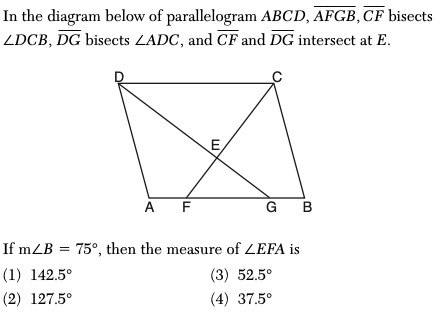
\includegraphics[width=11cm]{R-5images/R-5QuadrilateralsA.png}
\vspace{1cm}

\item Parallelogram properties\\
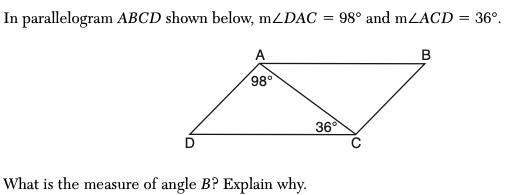
\includegraphics[width=12cm]{R-5images/R-5QuadrilateralsC.png}

\newpage
\item Parallelogram properties\\
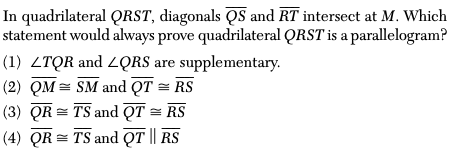
\includegraphics[width=12cm]{R-5images/R-5QuadrilateralsB.png}

\item Quadrilateral $MATH$ has both pairs of opposite sides congruent and parallel. Which statement about quadrilateral $MATH$ is always true?
\begin{enumerate}
    \item $\overline{MT} \cong \overline{AH}$
    \item $\overline{MT} \perp \overline{AH}$
    \item $\angle MHT \cong \angle ATH$
    \item $\angle MAT \cong \angle MHT$
\end{enumerate}

\item Parallelogram angle situation\\
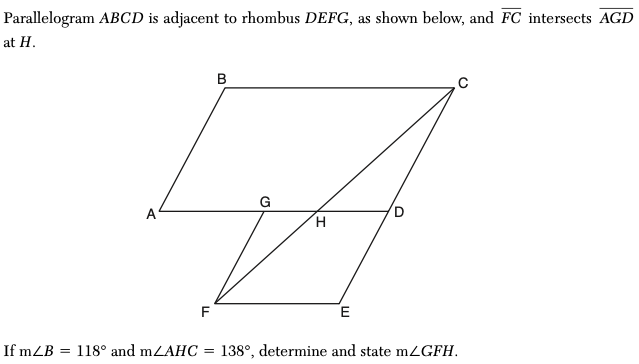
\includegraphics[width=14cm]{R-5images/R-5QuadrilateralsD.png}

\newpage
\item Parallelogram properties\\
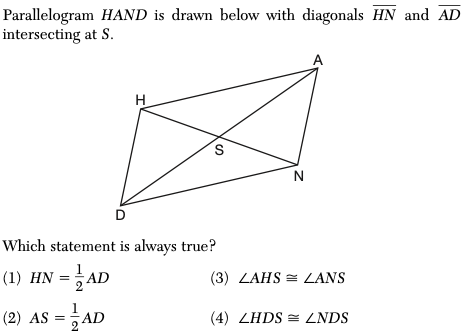
\includegraphics[width=11cm]{R-5images/R-5QuadrilateralsG.png}

\item Parallelogram angle situation\\
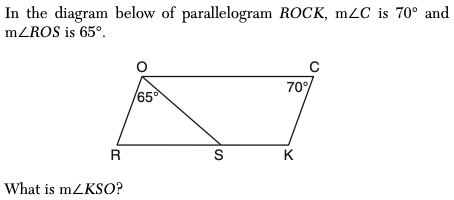
\includegraphics[width=11cm]{R-5images/R-5QuadrilateralsJ.png}
\vspace{1cm}

\item In parallelogram $ABCD$ shown below, the bisectors of $\angle ABC$ and $\angle DCB$ meet at $E$, a point on $\overline{AD}$.
\begin{center}
    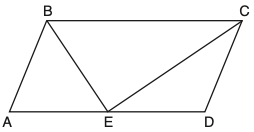
\includegraphics[width=6cm]{R-5images/R-5QuadrilateralsF.png}
\end{center}
If the m$\angle A=68^\circ$, determine and state the m$\angle BEC$.

\newpage
\item Given: Parallelogram $ABCD$ with diagonal $\overline{AC}$ drawn
\begin{center}
    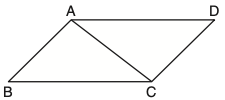
\includegraphics[width=6cm]{R-5images/R-5QuadrilateralsH.png}
\end{center}
Prove $\triangle ABC \cong \triangle CDA$
\vspace{3cm}

\item Parallelogram angle proof\\
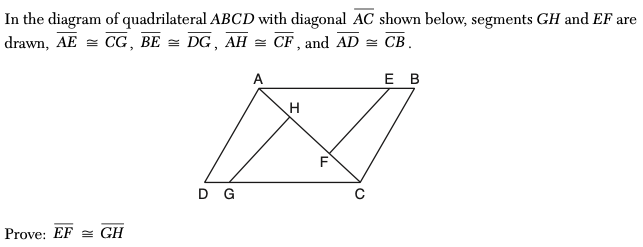
\includegraphics[width=16cm]{R-5images/R-5QuadrilateralsE.png}

\end{enumerate}
\end{document}
  